\documentclass[11pt,a4paper]{article}

\usepackage[T1]{fontenc}
\usepackage[utf8]{inputenc}
\usepackage{lmodern}
\usepackage{microtype}
\usepackage[margin=2.4cm]{geometry}
\usepackage{amsmath,amssymb}
\usepackage{graphicx}
\usepackage{booktabs}
\usepackage{tabularx}
\usepackage{array}
\usepackage{longtable}
\usepackage{enumitem}
\usepackage{float}
\usepackage[font=small,labelfont=bf]{caption}
\usepackage[dvipsnames]{xcolor}
\usepackage{fancyhdr}
\usepackage{titlesec}
\usepackage{hyperref}

\definecolor{accent}{HTML}{2A78D6}
\hypersetup{colorlinks=true,linkcolor=accent,urlcolor=accent,citecolor=accent}
\setlist{itemsep=2pt,topsep=4pt}
\setlength{\parskip}{4pt}
\setlength{\parindent}{0pt}
\titleformat{\section}{\Large\bfseries\color{accent}}{\thesection}{0.6em}{}
\titleformat{\subsection}{\large\bfseries}{\thesubsection}{0.5em}{}
\pagestyle{fancy}
\fancyhf{}
\lhead{\small sleepwatch: progress report, Phases 0--3b}
\rhead{\small 7 October 2026}
\cfoot{\small\thepage}
\renewcommand{\headrulewidth}{0.4pt}
\graphicspath{{figures/}}

\newcommand{\night}[2]{\texttt{Bidslab#1/#2}}
\newcommand{\code}[1]{\texttt{#1}}
\newcommand{\commit}[1]{\texttt{#1}}
\newcommand{\D}[1]{D#1}
\newcommand{\ci}[3]{$#1$ [$#2$, $#3$]}

\title{\textbf{sleepwatch}\\[4pt]\large Progress report: Phases 0--3b\\[2pt]
\normalsize Data, sleep staging, personalization and personalized anomaly detection}
\author{}
\date{7 October 2026\\[2pt]\small Repository state: \commit{main} at \commit{e7bbd1a}, in sync with GitHub}

\begin{document}
\maketitle
\thispagestyle{fancy}

\begin{abstract}
\noindent \textbf{The project.} sleepwatch uses the PhysioNet BIDSleep dataset: 47 healthy adults, 253 nights, with Apple
Watch heart rate and accelerometry and Dreem-2 EEG sleep stages corrected by an expert. It aims to
stage sleep from the watch, detect nights that differ from a person's own earlier nights, and
later ask follow-up questions about those nights.

\textbf{Staging.} A bidirectional GRU over whole nights reaches 5-class Cohen's kappa
\ci{0.510}{0.482}{0.537}, against $0.381$ for gradient-boosted trees.

\textbf{Personalization.} Five label-free ways of using a person's earlier nights did not improve
staging. Fine-tuning on the person's own labelled nights shows a person-specific signal, but only
a small, non-significant gain over the population model.

\textbf{Anomaly detection.} The personalized detector keeps false alarms on new people at 3.2\%,
but its recall of anomalies injected into the raw signals is low: 27\% for a whole-night
+10~bpm rise, 20\% for eight awakenings and 10\% for a 60-minute delay in sleep onset. The scores
respond (AUROC up to 0.82--0.91), but the pre-declared alarm rule places the threshold at the
edge of about 125 training nights. A post-hoc screen for heart-rate artifacts changed recall by at
most $+0.026$.

\textbf{Verification.} 111 automated tests pass, an independent review notebook passes 144 of
146 checks (both failures diagnosed), and every reported run comes from a clean commit and
reproduces exactly.
\end{abstract}

\vspace{4pt}
\noindent\fbox{\parbox{\dimexpr\linewidth-2\fboxsep-2\fboxrule}{\small
\textbf{How to read this report.}
\begin{itemize}[leftmargin=*]
\item \textbf{Purpose.} It is written so the work can be checked before Phase~4 starts.
\item \textbf{References.} Decision-log entries (\code{docs/decisions.md}) are cited as
\D{12}. Dataset details are in \code{docs/data.md}, and the full analyses in the notebooks under
\code{notebooks/}.
\item \textbf{Commit hashes.} They are the current ones. Hashes written before 2026-10-06 (in
run records, notebook outputs and older log entries) translate through
\code{docs/commit\_map.tsv} (Section~\ref{sec:problems}).
\end{itemize}}}

\newpage
\tableofcontents
\newpage

%-----------------------------------------------------------------------------------------------
\section{Summary}

\begin{table}[H]
\centering\small
\begin{tabularx}{\linewidth}{Xl}
\toprule
What & Result \\
\midrule
Staging, GRU, 5-class kappa (47 subjects, 253 nights) & \ci{0.510}{0.482}{0.537} \\
Staging, boosted trees, 5-class kappa & \ci{0.381}{0.357}{0.404} \\
Best label-free personalization vs its control & $-0.003$ (CI includes 0) \\
Fine-tuning on own labelled nights vs population GRU & $+0.004$ to $+0.014$ (CIs include 0) \\
Anomaly false alarms, clean test nights (157 nights) & \ci{3.2\%}{0.7}{6.1} \\
Anomaly recall, whole-night +10 bpm & \ci{0.27}{0.18}{0.37}; AUROC 0.82 \\
Anomaly recall, 8 awakenings & \ci{0.20}{0.13}{0.28}; AUROC 0.79 \\
Anomaly recall, onset +60 min & \ci{0.10}{0.05}{0.17}; AUROC 0.91 \\
Effect of the artifact screen on recall (Phase 3b) & $-0.006$ to $+0.026$ \\
\bottomrule
\end{tabularx}
\caption{Key numbers. Brackets are 95\% confidence intervals from resampling subjects.}
\end{table}

\begin{itemize}
\item \textbf{Data.} All 253 nights are checksum-verified and turned into 218,277 labelled 30-s
epochs with label-free features. Several data problems were found and documented:
  \begin{itemize}
  \item the expert labels appear to run about 90~s late;
  \item two nights have labels offset by 31 and 59~min;
  \item one night has interleaved heart-rate streams;
  \item two nights have likely heart-rate artifacts.
  \end{itemize}
\item \textbf{Staging} works at a typical level for wrist data. N1 remains the hard stage.
\item \textbf{Personalization of staging} is a negative result across Phases~2 and~2b.
\item \textbf{Anomaly detection.} The calibration carries over to new people, and the scores
separate injected from clean nights. Recall at the calibrated threshold is low, mainly because
of how strict the threshold rule turns out to be.
\end{itemize}

%-----------------------------------------------------------------------------------------------
\section{How the work was run}

\begin{itemize}
\item \textbf{Phase gates.} Each phase started with a plan you approved and ended with a summary
and a wait for your go-ahead. Decisions that were yours are marked \emph{user decision} in the
log.
\item \textbf{Protocol before results.} For Phases~2b, 3 and~3b, the designs, controls, grids
and metrics were committed to the decision log \emph{before} any run. Outcomes were recorded
afterwards in separate entries (\D{40}, \D{46}, \D{48}), without changing the protocol.
\item \textbf{No tuning on test subjects.}
  \begin{itemize}
  \item \textbf{Splits:} all splits are by subject, with one fold file created once and never
  changed.
  \item \textbf{Training-subject choices:} hyperparameters, early stopping, shrinkage strengths
  and alarm thresholds come only from training subjects, often through inner splits.
  \item \textbf{Post-hoc findings:} anything found by looking at test results is labelled a
  diagnostic or a post-hoc analysis and changes no headline number.
  \end{itemize}
\item \textbf{Provenance.} Every run writes its resolved config, git commit, a dirty flag and its
metrics to \code{results/<experiment>/<timestamp>/}. Reported runs must come from a clean tree.
\item \textbf{Independent review.} \code{notebooks/phase1\_2\_check.ipynb} re-derives the main
claims, often without the pipeline code (Section~\ref{sec:verification}).
\end{itemize}

%-----------------------------------------------------------------------------------------------
\section{Phase 0: setup (30 September)}

\begin{itemize}
\item \textbf{Layout} (\D{1}, \D{2}).
  \begin{itemize}
  \item \textbf{Repository:} on the internal disk.
  \item \textbf{Data:} on the external T7 drive, which is exFAT, so no symlinks or virtual
  environments can live there. \code{data/raw} and \code{data/interim} are symlinks into it.
  \item \textbf{Ignored outputs:} \code{data/} and \code{results/} are gitignored, and a
  pre-commit hook refuses data files.
  \end{itemize}
\item \textbf{Tooling} (\D{4}, \D{5}, \D{12}).
  \begin{itemize}
  \item \textbf{Environment:} uv with a lockfile, on Python~3.12.
  \item \textbf{Quality tools:} ruff, pytest and pre-commit.
  \item \textbf{CI:} GitHub Actions runs lint and the tests that need no data.
  \item \textbf{Settings:} paths come from environment variables, and experiment defaults from
  \code{configs/base.yaml}.
  \end{itemize}
\item \textbf{Dataset verification.} The first local download was silently incomplete: only 9 of
47 subjects were intact, and the last file was NUL-padded. Loaders now read only nights whose
files match PhysioNet's \code{SHA256SUMS.txt} (\D{3}). The unzipped archive passes all 761
checksums (\D{20}).
\item \textbf{Evaluation protocol} (\D{7}).
  \begin{itemize}
  \item \textbf{Splits:} subject-level 5-fold \code{GroupKFold}.
  \item \textbf{Reporting:} pooled and per-subject metrics with subject-bootstrap CIs.
  \item \textbf{Personalization:} scored on fixed evaluation nights, night~4 onward for the 43
  subjects with at least 4 nights (112 nights).
  \end{itemize}
\item \textbf{Personalization rule} (\D{8}). The headline variants must work without labels,
because a real user has no EEG labels. Anything using labels is an upper bound.
\end{itemize}

%-----------------------------------------------------------------------------------------------
\section{Phase 1: data pipeline, features and exploration (30 September -- 1 October)}

\subsection{What was built}
\begin{itemize}
\item \textbf{Loader} (\code{data/loader.py}).
  \begin{itemize}
  \item Reads a night's heart rate, accelerometer and both label sets.
  \item Converts \code{recStart} from US Eastern local time.
  \item Crops the signals to the label window.
  \item Skips and counts malformed rows (\D{21}).
  \end{itemize}
\item \textbf{Epoch features} (\code{features/epoch\_features.py},
\code{configs/features/v1.yaml}).
  \begin{itemize}
  \item \textbf{Grids:} heart rate on a 1~Hz grid and motion on a 50~Hz grid, with gaps never
  bridged (\D{15}).
  \item \textbf{Heart-rate features:} level, spread, night-relative value, detrended value and
  first difference.
  \item \textbf{Motion features:} ENMO, band-passed activity and arm angle.
  \item \textbf{Time:} time since start and since an actigraphy-estimated sleep onset.
  \item \textbf{Context:} centred rolling windows.
  \end{itemize}
\item \textbf{What the features exclude.}
  \begin{itemize}
  \item \textbf{Labels:} a test checks that shuffling the labels leaves every feature unchanged
  (\D{17}).
  \item \textbf{Coverage columns:} these are kept out of the model inputs, because the
  heart-rate sample count is about 7\% lower during Wake, which would be a device shortcut
  (\D{16}, \D{31}).
  \end{itemize}
\item \textbf{Epoch table:} 218,277 epochs, with a per-night quality table.
\end{itemize}

\subsection{What the exploration found}
\begin{itemize}
\item \textbf{Coverage.} 2.7\% of epochs have no heart rate and 5.0\% no motion. 44 nights are
under 90\% coverage on one signal, and on 12 nights the watch stopped about an hour before the
labels end.
\item \textbf{Stage mix.} Wake 11\%, N1 7\%, N2 37\%, N3 18\%, REM 26\%. N3 comes early and REM
late, so time of night is informative and also a confound.
\item \textbf{Heart rate is mainly about the person} (Figure~\ref{fig:hr}). Subject medians range
from 52 to 82~bpm, far more than the differences between stages. This motivated the personal
baselines of Phase~3.
\item \textbf{Dreem vs expert labels.} Kappa is 0.75 (5-class). Since the expert labels are
corrections of Dreem's, this is not independent agreement.
\item \textbf{The expert labels appear about 90~s late} (Figure~\ref{fig:timing}). Movement and
heart rate separate expert-Wake best when the labels are paired with the signals three epochs
earlier, consistently and without drift. Dreem's labels line up within one epoch.
\emph{User decision} (\D{22}): keep the documented alignment for headline results, and run a
shifted-label sensitivity analysis.
\item \textbf{\night{01}{4}.} Its expert and Dreem labels disagree completely (kappa $-0.03$).
Phase~2 later showed that the watch models agree with the expert labels at a typical level, so
the Dreem file is the odd one out. \emph{User decision} (\D{23}): keep the night.
\item \textbf{\night{06}{2}} alternates between two heart-rate levels, apparently two
interleaved streams. It is flagged, not corrected (\D{24}).
\end{itemize}

\begin{figure}[H]
\centering
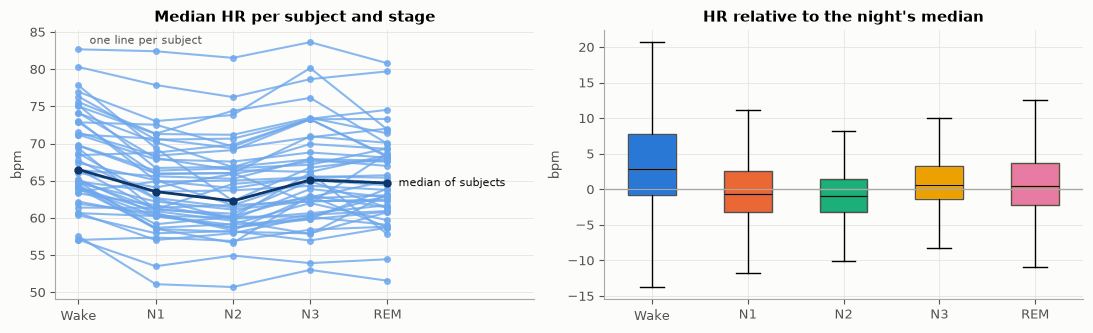
\includegraphics[width=\linewidth]{eda_hr_by_stage}
\caption{Heart rate by stage (notebook \code{01\_eda}). Left: each subject's median heart rate
per stage; the spread between people dwarfs the differences between stages. Right: heart rate
relative to the night's median.}
\label{fig:hr}
\end{figure}

\begin{figure}[H]
\centering
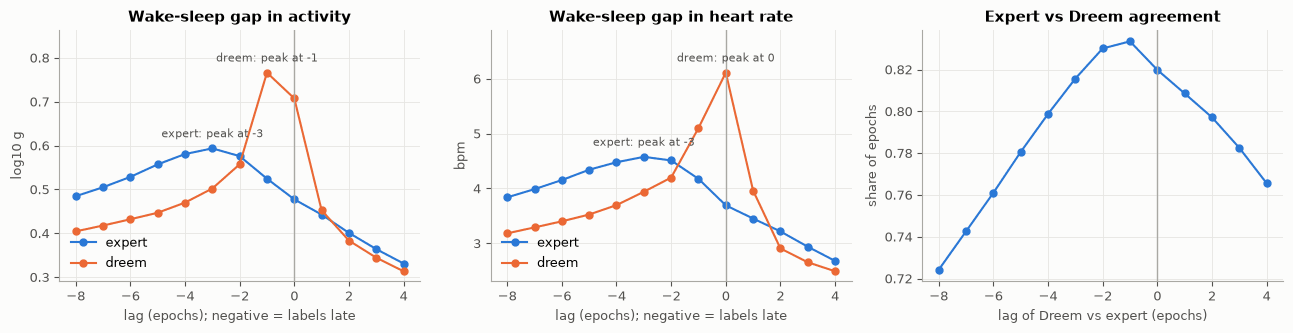
\includegraphics[width=\linewidth]{eda_label_timing}
\caption{Label timing (notebook \code{01\_eda}). The Wake--sleep gap in activity and heart rate
peaks when the expert labels are paired with signals three epochs earlier; Dreem's peaks at
$-1$ and~0. Right: the expert labels also match Dreem best when shifted by 1--2 epochs.}
\label{fig:timing}
\end{figure}

%-----------------------------------------------------------------------------------------------
\section{Phase 2: sleep staging (1 October)}

\subsection{Models}
\begin{itemize}
\item \textbf{Gradient-boosted trees, per epoch} (scikit-learn
\code{HistGradientBoostingClassifier}, \D{25}). A 6-point grid and early stopping on held-out
training subjects (\D{26}), with balanced class weights chosen by validation macro-F1.
\item \textbf{Bidirectional GRU over whole nights.} One 48-unit layer, sized on fold~0's
validation subjects (\D{27}), with an unweighted loss.
  \begin{itemize}
  \item \textbf{Implementation:} two forward GRUs, one over the reversed night. It is tested
  equal to PyTorch's bidirectional GRU to $10^{-6}$, and is 3$\times$ faster.
  \item \textbf{Hardware:} you asked for the Apple GPU (MPS). I measured it at about 4$\times$
  \emph{slower} for this sequential model, so it trains on CPU, folds in parallel, by your
  choice (\D{32}).
  \end{itemize}
\end{itemize}

\subsection{Results}
\begin{table}[H]
\centering\small
\begin{tabular}{lcccc}
\toprule
Model & Kappa, 5-class [95\% CI] & Macro-F1 & Kappa, 4-class & Accuracy, 4-class \\
\midrule
GRU & \ci{0.510}{0.482}{0.537} & 0.566 & 0.533 & 0.684 \\
Boosted trees & \ci{0.381}{0.357}{0.404} & 0.504 & 0.390 & 0.592 \\
\bottomrule
\end{tabular}
\caption{Population staging models, 5-fold cross-validation by subject (47 subjects, 253
nights).}
\end{table}

\begin{itemize}
\item \textbf{GRU vs trees.} The paired difference is \ci{+0.129}{+0.113}{+0.145}. The GRU is
better on every stage except N1: F1 0.155 vs 0.236 (Figure~\ref{fig:confusion}).
\item \textbf{Spread.} Per-subject kappa is $0.506 \pm 0.096$ (range 0.247--0.662).
\item \textbf{Calibration} is usable as is: ECE is 0.037 for the GRU and 0.048 for the trees.
\item \textbf{Robustness.} Re-pairing the labels by the $\sim$90~s offset changes kappa by at
most 0.012. Training on Dreem labels instead of the expert's changes it by
\ci{-0.003}{-0.010}{+0.005}.
\item \textbf{Context.} The dataset authors report 71\% 4-class accuracy, under a different
protocol and with a sampling-rate input excluded here. The two are not directly comparable.
\end{itemize}

\begin{figure}[H]
\centering
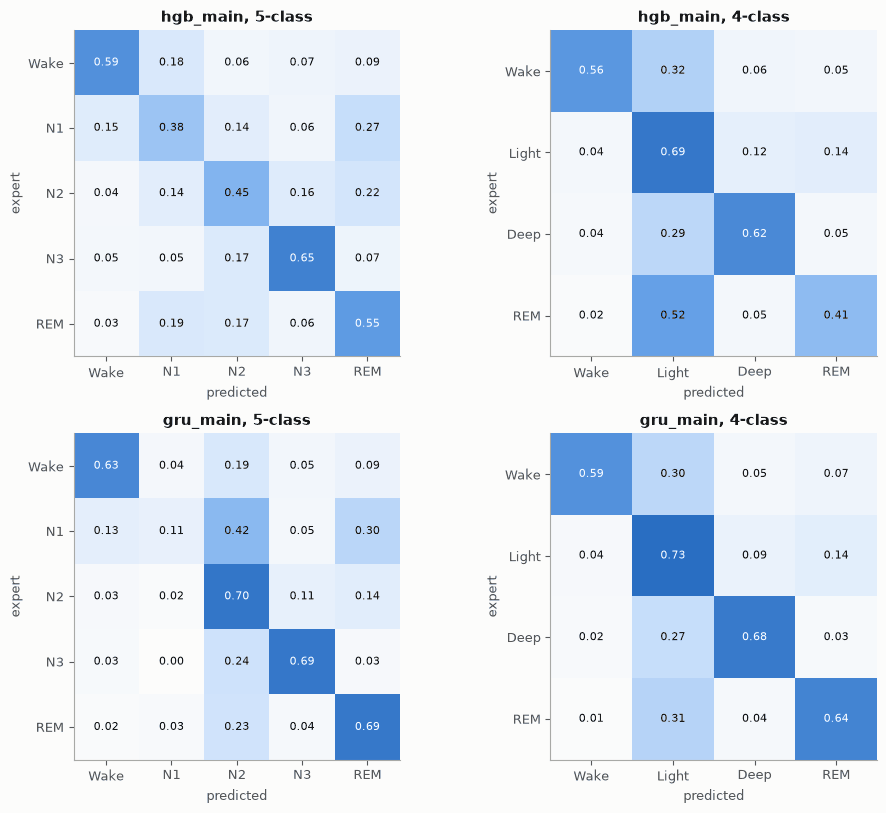
\includegraphics[width=0.78\linewidth]{staging_confusion}
\caption{Confusion matrices, rows normalized by the expert stage (notebook \code{02\_staging}).
The GRU classes only 11\% of N1 epochs as N1, mostly confusing it with N2 and REM.}
\label{fig:confusion}
\end{figure}

\subsection{Personalization}
\begin{itemize}
\item \textbf{The question.} Do 1--3 earlier nights of the same person help?
\item \textbf{Features tested} (\D{28}, \D{29}).
  \begin{itemize}
  \item \code{prior\_norm}: label-free per-person statistics.
  \item \code{prior\_stage}: per-stage statistics from the earlier nights' expert labels, as an
  upper bound.
  \end{itemize}
\item \textbf{Control.} A model that uses $N$ earlier nights can only train on the nights after
them. The control therefore trains on exactly the same nights, without the personal features.
\item \textbf{Result} (Figure~\ref{fig:pers}).
  \begin{itemize}
  \item \code{prior\_norm} changed kappa by $-0.020$ to $-0.003$ for the GRU and $-0.003$ to
  $0.000$ for the trees. Every CI includes~0.
  \item \code{prior\_stage} gained at most $+0.012$ for the trees (CI [0.004, 0.022]) and lost
  0.029--0.040 for the GRU.
  \end{itemize}
\item \textbf{Reported as a negative result} (\D{34}), not redesigned.
\end{itemize}

\begin{figure}[H]
\centering
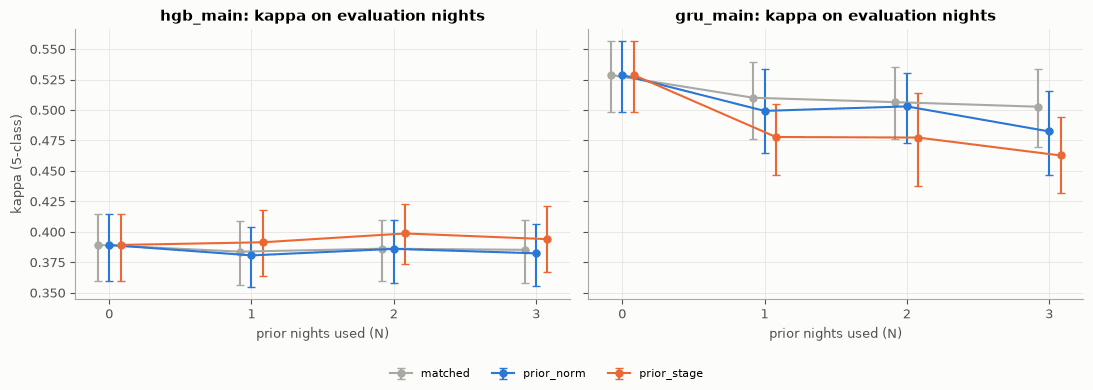
\includegraphics[width=\linewidth]{staging_personalization}
\caption{Kappa on the fixed evaluation nights by number of earlier nights used (notebook
\code{02\_staging}). The matched control (grey) falls too, because fewer nights remain for
training.}
\label{fig:pers}
\end{figure}

\textbf{Found along the way.} On \night{42}{1} and \night{68}{2} the labels start when the watch
starts, 31 and 59~min after \code{recStart}.
\begin{itemize}
\item \textbf{Phase~2.} The finding came from test predictions, so both nights stay in every
Phase~2 result (\D{33}). Excluding them would raise kappa by 0.003--0.005.
\item \textbf{Phase~3.} You decided to exclude them there.
\end{itemize}

%-----------------------------------------------------------------------------------------------
\section{Phase 2b: three more personalization designs (1--2 October)}

You asked to test three more designs before Phase~3. The protocol was committed before any run
(\D{35}--\D{38}).

\begin{table}[H]
\centering\small
\begin{tabularx}{\linewidth}{>{\raggedright\arraybackslash}Xc>{\raggedright\arraybackslash}p{4.2cm}l}
\toprule
Design & Labels? & Compared with & Kappa difference [95\% CI] \\
\midrule
A: baseline from all earlier nights, trees & no & population model & \ci{-0.004}{-0.011}{+0.004} \\
A: same, GRU & no & population model & \ci{-0.007}{-0.019}{+0.005} \\
B: learned summary of earlier nights & no & same model, another person's nights & \ci{-0.006}{-0.025}{+0.018} \\
C: fine-tuning on own nights ($N$ = 1, 2, 3, all) & yes & fine-tuning on another person's nights & $+0.022$ to $+0.035$ (CIs $>0$) \\
C: same & yes & population GRU & $+0.004$ to $+0.014$ (CIs include 0) \\
\bottomrule
\end{tabularx}
\caption{Phase 2b primary results on the fixed evaluation nights.}
\end{table}

\begin{figure}[H]
\centering
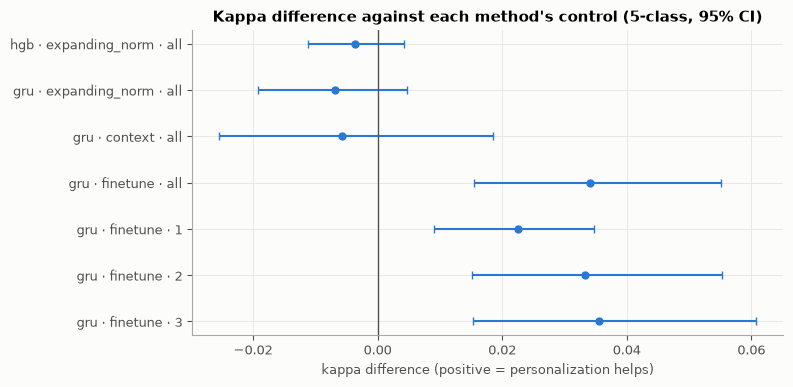
\includegraphics[width=0.75\linewidth]{p2b_primary}
\caption{Kappa difference against each method's control (notebook
\code{02b\_personalization}).}
\end{figure}

\begin{itemize}
\item \textbf{Design~B carried no personal information.} It scored no better with the person's
own nights than with someone else's, and showed no sign of memorizing training subjects.
\item \textbf{Fine-tuning's control is not neutral.} Fine-tuning on another person's nights
\emph{costs} 0.018--0.026 kappa. That is why the own-vs-other difference looks larger than the
gain over doing nothing.
\item \textbf{Reproducibility.} All Phase~2 experiments were rerun at the Phase~2b commit
(\commit{eea3ee1}) and reproduced their earlier predictions exactly (\D{39}).
\item \textbf{Conclusion.} Across Phases~2 and~2b, no label-free design helped. The
person-specific signal appears only with EEG-scored labels of the person's own nights, and
even then the net gain is small.
\end{itemize}

%-----------------------------------------------------------------------------------------------
\section{Phase 3: personalized anomaly detection (5--6 October)}
\label{sec:phase3}

\emph{User decisions:}
\begin{itemize}
\item stages come from the population GRU, with expert stages as a best case and a stage-free
detector as the simplest comparison;
\item the two offset nights are excluded.
\end{itemize}
The protocol was committed before any run (\D{41}--\D{45}).

\subsection{Detector}
For person $p$, sleep stage $s$ and time-of-night bin $t$, the expected value of each epoch
signal (heart rate, $\log_{10}$ activity) is
\[
\hat{x}_{p,s,t} \;=\; \mu_{s,t} \;+\; b_p \;+\; b_{p,s}.
\]
\begin{itemize}
\item \textbf{Population term.} $\mu_{s,t}$ is the training subjects' mean.
\item \textbf{Personal offsets.} $b_p$ and $b_{p,s}$ are averages of per-night mean residuals
over the person's \emph{strictly earlier} nights. Each is shrunk by $N/(N+\kappa)$, with
$\kappa$ estimated on training subjects by the method of moments.
\item \textbf{Epoch score.} $z = (x - \hat{x})/\sigma_s$, with a per-stage residual SD
$\sigma_s$.
\item \textbf{Four night channels,} each one-sided in the ``worse'' direction:
\begin{enumerate}[nosep]
\item the highest 30-min mean heart-rate $z$;
\item the whole-night mean heart-rate $z$;
\item wake bouts per hour, $z$-scored against the person's earlier nights;
\item onset latency, $z$-scored in the same way.
\end{enumerate}
\item \textbf{Null.} The training subjects' clean nights, scored out of sample through 5 inner
folds that each have their own GRU.
\item \textbf{Tail probability.} Each channel value $v$ gets
$p = (1+\#\{\text{null} \ge v\})/(1+n)$.
\item \textbf{Alarm.} A night is flagged when $\min p$ is at or below the largest threshold whose
leave-one-out rate on the null is at most 5\%.
\item \textbf{Detectors.} Stages (GRU, expert, none) $\times$ baseline (personal,
population-only) gives 6 detectors. The primary one is GRU stages with the personal baseline.
\item \textbf{Scope.} 157 test nights from 47 subjects, each with at least 2 earlier usable
nights.
\end{itemize}

\begin{figure}[H]
\centering
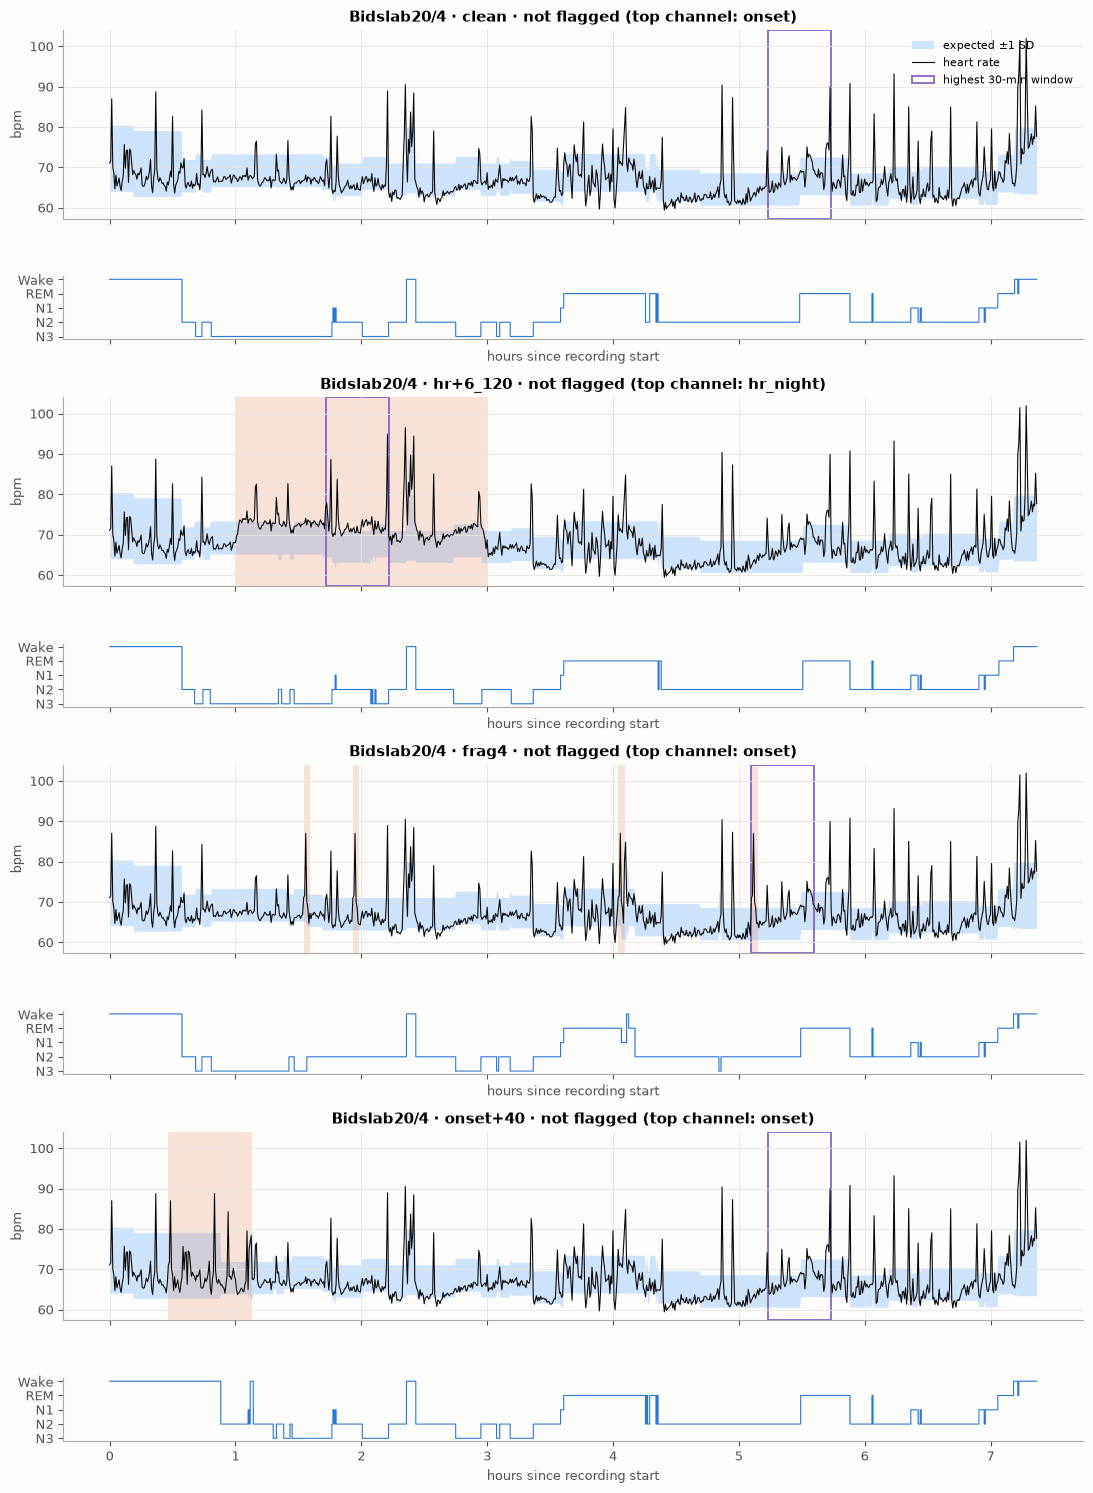
\includegraphics[width=0.82\linewidth]{anomaly_detector_view}
\caption{What the detector sees (notebook \code{03\_anomaly}). Each panel shows one night: heart
rate against the personal expectation ($\pm$1~SD band), with the predicted hypnogram below it.
Panels: a clean night, then three injected versions of it (HR +6~bpm for 2~h, four awakenings,
onset +40~min), with the injected stretches shaded. None of the four is flagged.}
\label{fig:view}
\end{figure}

\subsection{Validation by injection}
\begin{itemize}
\item \textbf{What was injected} into the \emph{raw} signals of test nights:
  \begin{itemize}
  \item \textbf{heart rate:} +3, +6 or +10~bpm for 30~min, 2~h or the whole sleep period, with
  2-min ramps;
  \item \textbf{fragmentation:} 2, 4 or 8 three-minute awakenings copied from the same night's
  wake;
  \item \textbf{delayed onset:} +20, +40 or +60~min.
  \end{itemize}
\item \textbf{How.} Features were rebuilt with the unchanged pipeline, and stages were
re-predicted.
\item \textbf{Volume.} 2,337 injected versions. Three nights had no wake to copy from, so they
got heart-rate injections only.
\item \textbf{Integrity.} All 157 rebuilt clean nights matched the stored features and stages.
\end{itemize}

\subsection{Results}
\begin{table}[H]
\centering\small
\begin{tabular}{lcccc}
\toprule
Injected anomaly & Recall [95\% CI] & AUROC & Recall, 3b & 3b $-$ 3 [95\% CI] \\
\midrule
HR +3 bpm, 30 min & \ci{0.03}{0.01}{0.06} & 0.50 & 0.03 & \ci{+0.000}{-0.018}{+0.019} \\
HR +3 bpm, 2 h & \ci{0.04}{0.01}{0.08} & 0.53 & 0.04 & \ci{-0.006}{-0.030}{+0.013} \\
HR +3 bpm, whole night & \ci{0.04}{0.01}{0.08} & 0.60 & 0.04 & \ci{+0.000}{-0.018}{+0.019} \\
HR +6 bpm, 30 min & \ci{0.03}{0.01}{0.05} & 0.52 & 0.03 & \ci{+0.006}{0.000}{+0.020} \\
HR +6 bpm, 2 h & \ci{0.04}{0.01}{0.08} & 0.58 & 0.04 & \ci{+0.000}{-0.018}{+0.019} \\
HR +6 bpm, whole night & \ci{0.08}{0.03}{0.14} & 0.70 & 0.10 & \ci{+0.013}{-0.012}{+0.037} \\
HR +10 bpm, 30 min & \ci{0.04}{0.01}{0.08} & 0.58 & 0.04 & \ci{+0.000}{-0.018}{+0.019} \\
HR +10 bpm, 2 h & \ci{0.08}{0.04}{0.14} & 0.69 & 0.10 & \ci{+0.019}{0.000}{+0.043} \\
HR +10 bpm, whole night & \ci{0.27}{0.18}{0.37} & 0.82 & 0.29 & \ci{+0.013}{0.000}{+0.031} \\
2 awakenings & \ci{0.04}{0.01}{0.07} & 0.58 & 0.04 & \ci{+0.000}{-0.019}{+0.019} \\
4 awakenings & \ci{0.05}{0.02}{0.09} & 0.66 & 0.06 & \ci{+0.006}{0.000}{+0.020} \\
8 awakenings & \ci{0.20}{0.13}{0.28} & 0.79 & 0.23 & \ci{+0.026}{+0.006}{+0.053} \\
Onset +20 min & \ci{0.03}{0.01}{0.06} & 0.67 & 0.05 & \ci{+0.013}{0.000}{+0.033} \\
Onset +40 min & \ci{0.04}{0.01}{0.07} & 0.83 & 0.06 & \ci{+0.019}{0.000}{+0.043} \\
Onset +60 min & \ci{0.10}{0.05}{0.17} & 0.91 & 0.13 & \ci{+0.026}{+0.006}{+0.051} \\
\midrule
\emph{False alarms (clean nights)} & \ci{0.032}{0.007}{0.061} & & 0.032 & $+0.000$ \\
\bottomrule
\end{tabular}
\caption{Primary detector (GRU stages, personal baseline), Phase~3 and the Phase~3b rescore
(Section~\ref{sec:phase3b}). Heart-rate conditions cover 157 nights; fragmentation and onset
cover 154.}
\label{tab:anomaly}
\end{table}

\begin{figure}[H]
\centering
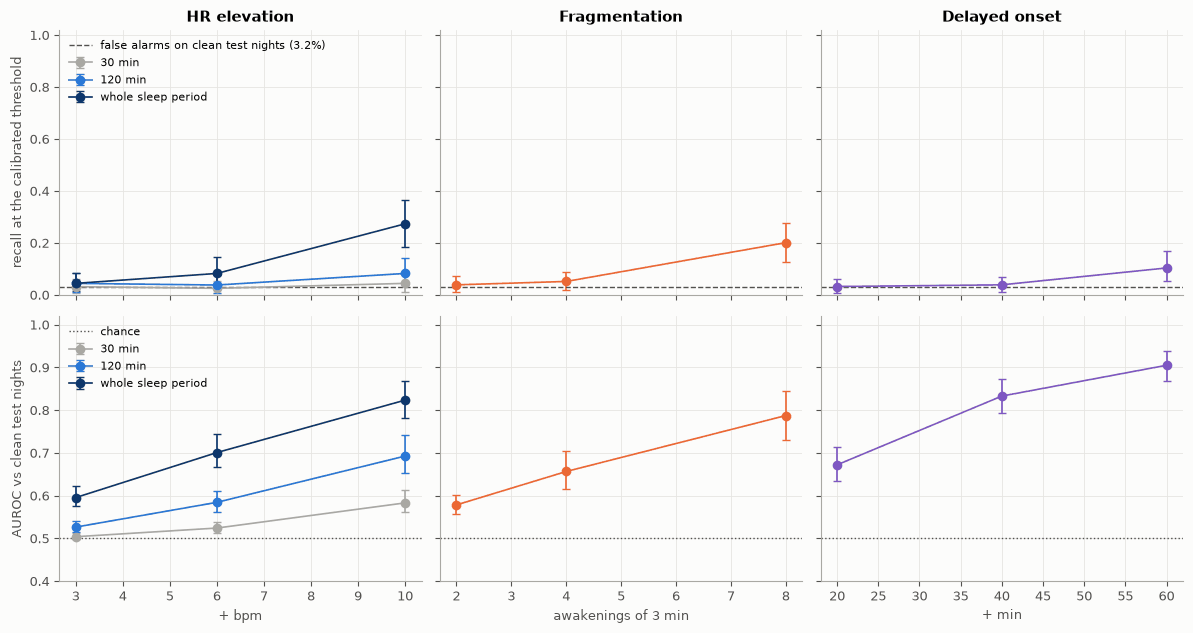
\includegraphics[width=\linewidth]{anomaly_recall_auroc}
\caption{Recall at the calibrated threshold (top) and AUROC (bottom) by anomaly type and size
(notebook \code{03\_anomaly}). The dashed line is the false-alarm rate on clean test nights.}
\label{fig:recall}
\end{figure}

\begin{itemize}
\item \textbf{False alarms carry over to new people.} All six detectors stay at 2.5--4.5\%; the
training null rates were 2.5--4.8\%.
\item \textbf{The personal baseline helps only where people differ in level.} Against the
population-only baseline:
  \begin{itemize}
  \item whole-night +10~bpm: recall \ci{+0.17}{0.11}{0.24} and AUROC 0.82 vs 0.70;
  \item elsewhere: at most $+0.03$, and the other CIs include~0.
  \end{itemize}
\item \textbf{Staging is the bottleneck for fragmentation.} With expert stages, 8 awakenings are
caught 63\% of the time, against 20\% with GRU stages (difference \ci{-0.43}{-0.53}{-0.33}).
The GRU marks a wake bout over only 57\% of the inserted awakenings.
\item \textbf{The stage-free detector catches more whole-night heart-rate changes} (36\% vs
27\%). It does so at a higher false-alarm rate (4.5\%) and with a similar AUROC (0.84), so the
gap is mostly its operating point.
\item \textbf{Why recall is low} (post hoc).
  \begin{itemize}
  \item \textbf{The threshold sits at the edge of the null.} Tail probabilities move in steps of
  $1/(n+1)$ with $n \approx 125$, and four channels compete. In practice a test night must
  beat \emph{all}, or all but one, of the training nights in some channel.
  \item \textbf{The injections fall short of that edge.} The largest move their channel by
  2--3~$z$. That reaches the training nights' 95th percentile (1.6--3.0) but not their maximum
  (3.1--5.9).
  \item \textbf{In three folds an artifact sets the edge.} \night{43}{3} sets the 30-min
  heart-rate edge there (Figure~\ref{fig:artifact}).
  \end{itemize}
\item \textbf{Real nights.} 5 of 157 clean test nights were flagged, about what chance alone
would give:
  \begin{itemize}
  \item \night{11}{3} and \night{66}{3}: heart rate above the personal band for most of the
  night;
  \item \night{22}{6}: heart rate rising by about 18~bpm over the first 1.5~h;
  \item \night{32}{6}: an onset latency of 108~min;
  \item \night{43}{3}: the artifact.
  \end{itemize}
They are described, with no causes inferred. Each flagged night also gets a structured
JSON summary (\code{AnomalySummary}), the planned input for the Phase~4 agent.
\end{itemize}

\begin{figure}[H]
\centering
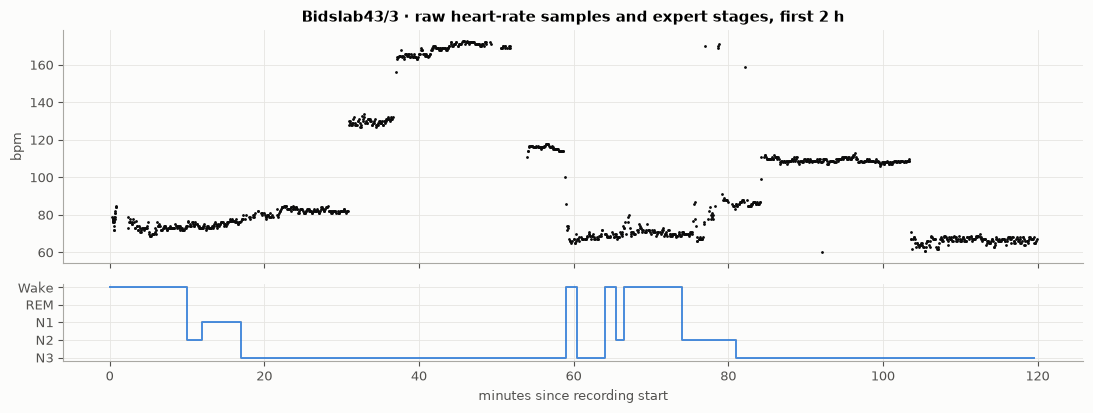
\includegraphics[width=\linewidth]{anomaly_artifact_43_3}
\caption{\night{43}{3}, raw heart-rate samples and expert stages, first 2~h (notebook
\code{03\_anomaly}). Heart rate sits flat at about 130, 170 and 110~bpm, with jumps of up to
94~bpm between readings seconds apart, while the EEG shows deep sleep. It is almost certainly a
measurement artifact.}
\label{fig:artifact}
\end{figure}

\textbf{Operational note.} The first full run crashed after 33~min: the lid was closed on battery,
which \code{caffeinate} cannot prevent, so the T7 lost power and a file read failed. Nothing was
saved. The rerun on AC power took 57~min (30 GRU trainings, 2,337 nights rebuilt from raw data),
from a clean commit (\commit{eb5c420}).

%-----------------------------------------------------------------------------------------------
\section{Phase 3b: heart-rate artifact screen (6 October, post hoc)}
\label{sec:phase3b}

You chose a short follow-up to measure what removing such artifacts changes. The protocol was
committed before the run (\D{47}).

\begin{itemize}
\item \textbf{Rule (label-free).} An epoch is suspect if its heart rate is at least 40~bpm above
the night's median for at least 5 consecutive minutes. Its heart rate is then treated as missing
everywhere the detector looks: priors, nulls, baselines and test nights.
\item \textbf{How the rule was set.} The thresholds were chosen after seeing \night{43}{3}, from
the label-free heart-rate distribution, never from detector results.
\item \textbf{What it marks.} 2 of 251 usable nights: \night{43}{3} (41~min) and \night{53}{3}
(6~min, the same step--plateau--step pattern).
\item \textbf{Method.} The Phase~3 run was \emph{rescored}, reusing its stages, inner folds and
injected nights, so the screen is the only difference. Without the screen, the rescoring
reproduces Phase~3's scores and summaries exactly.
\item \textbf{Result} (Table~\ref{tab:anomaly}, Figure~\ref{fig:screen}).
  \begin{itemize}
  \item \textbf{False alarms:} unchanged at 3.2\%.
  \item \textbf{Recall:} changes by $-0.006$ to $+0.026$ per condition.
  \item \textbf{AUROC:} within 0.012.
  \end{itemize}
\item \textbf{Two effects partly cancel.} The artifact no longer makes \night{43}{3}'s versions
flag (11 of 16 before, 3 after), and the edge loosens slightly in some folds. The artifact was
not what kept recall low.
\item \textbf{Real nights.} \night{43}{3} dropped out and \night{34}{3} came in
(Figure~\ref{fig:staging-error}). The expert labels show the person awake throughout the flagged
window, but the GRU staged it as sleep, so waking heart rate was compared with sleep-level
expectations. Staging errors can therefore also produce flags.
\item \textbf{One pre-declared check failed, and was diagnosed.} In 5 injected versions of
\night{43}{3}, 10--18 artifact epochs stay unmasked. The rule's threshold follows the night's
median, which a 2-h injection raises, and an inserted awakening can split the artifact's run.
\item \textbf{The headline stays Phase~3's.} \code{anomaly\_main} remains the headline result.
\end{itemize}

\begin{figure}[H]
\centering
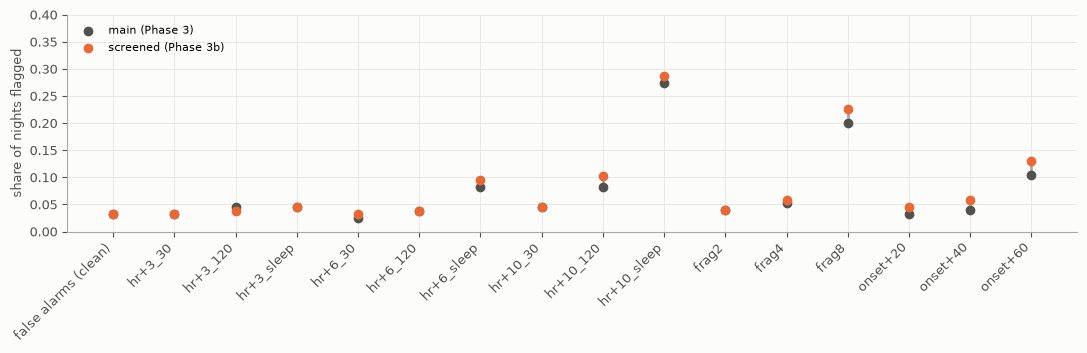
\includegraphics[width=\linewidth]{screen_main_vs_screened}
\caption{Share of nights flagged, Phase~3 (grey) vs Phase~3b (orange), primary detector (notebook
\code{03b\_screen}).}
\label{fig:screen}
\end{figure}

\begin{figure}[H]
\centering
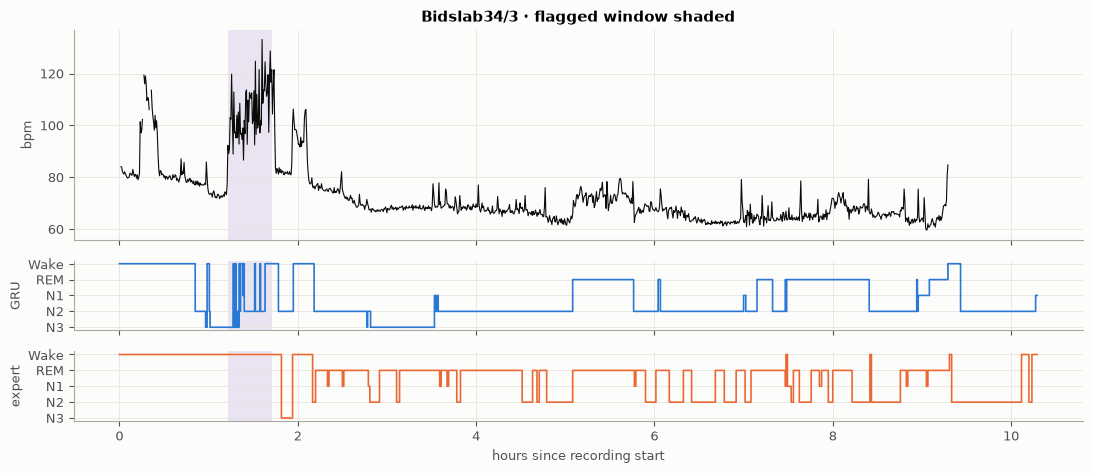
\includegraphics[width=\linewidth]{screen_34_3}
\caption{\night{34}{3}, newly flagged after the screen (notebook \code{03b\_screen}). In the
flagged window (shaded) the expert labels show Wake, but the GRU staged most of it as sleep.}
\label{fig:staging-error}
\end{figure}

%-----------------------------------------------------------------------------------------------
\section{Verification}
\label{sec:verification}

\begin{itemize}
\item \textbf{Automated tests: 111, all passing.} They cover synthetic-data logic and real-data
invariants:
  \begin{itemize}
  \item alignment, feature invariance across sampling rates, and no label leakage;
  \item metrics;
  \item the GRU against PyTorch's reference;
  \item the personalization controls;
  \item baselines that use only earlier nights, the shrinkage limits, and injections that land
  exactly where stated;
  \item thresholds that come only from other people;
  \item rescoring that reproduces a run exactly.
  \end{itemize}
\item \textbf{Review notebook: 144 of 146 checks pass.} Many checks re-implement claims
independently of the pipeline code. Its 18 sections cover:
  \begin{itemize}
  \item \textbf{data and Phase~1:} provenance, dataset integrity, raw formats, label and motion
  alignment, leakage and invariants, sampling-rate invariance, the label-timing finding (with
  positive controls), Dreem--expert agreement, and the numbers quoted in the docs;
  \item \textbf{Phase~2:} the runs, folds, recomputed metrics, personalization checks and
  reproducibility;
  \item \textbf{Phases~3 and~3b};
  \item \textbf{the test suite}.
  \end{itemize}
\item \textbf{The two failures.}
  \begin{itemize}
  \item \textbf{\night{06}{2}.} An independent re-alignment of heart rate differs from the
  pipeline's epoch values by a median of 0.55~bpm, against a 0.5 limit. This is not
  misalignment, since the unshifted pairing is clearly best. The night's interleaved heart-rate
  levels make a time-weighted mean and a plain mean differ more than usual.
  \item \textbf{The Phase~3b check on \night{43}{3}} (Section~\ref{sec:phase3b}).
  \end{itemize}
\item \textbf{Reproducibility.}
  \begin{itemize}
  \item All Phase~2 reruns reproduce the earlier predictions exactly.
  \item The Phase~3 rescoring reproduces Phase~3 exactly.
  \item A test checks that GRU predictions don't depend on how many folds run in parallel.
  \end{itemize}
\end{itemize}

%-----------------------------------------------------------------------------------------------
\section{Problems, mistakes and corrections}
\label{sec:problems}

These are listed so you can judge them. None changed a reported result after the fact.

\begin{enumerate}
\item \textbf{Incomplete first download} (Phase~0). It was caught by the checksums, which led to
the verified-nights-only rule.
\item \textbf{The wrong night named as the 2-s heart-rate night.} A quality statistic pointed to
\night{00}{2} instead of \night{06}{2}. The review notebook caught it, and the docs were
corrected (\D{24}).
\item \textbf{An overstated claim in \code{docs/data.md}} (Phase~2). It said the best label lag
is within $\pm 3$ epochs on the other nights. That holds for only 203 of 251, so it was
corrected to ``the best lag gains at most 0.06 kappa''.
\item \textbf{Two bugs in the Phase~2b code.} Validation-score unpacking was wrong, and a test
compared floats for exact equality. Both were fixed before any reported result.
\item \textbf{The Phase~3 protocol was loosely stated in two places.}
  \begin{itemize}
  \item \D{42} calls the threshold ``the 5th percentile''. The code, fixed before the run, uses
  ``the largest threshold with a leave-one-out rate $\le$ 5\%''.
  \item The AUROC pools test nights rather than pairing them per night.
  \end{itemize}
  The protocol also estimated 5 skipped nights; there were 3. All of this is recorded in
  \D{46}.
\item \textbf{Three bugs in the review checks} (not in the pipeline).
  \begin{itemize}
  \item A Phase~2 provenance check failed merely because a new package had been added.
  \item The heart-rate injection check counted epochs without heart rate as mismatches. The
  injections themselves are exact to $4\times10^{-14}$.
  \item The Phase~3 provenance check failed on Phase~3b's intended code changes.
  \end{itemize}
  Each check was rescoped to what matters, without loosening it: the code that produced the
  results must be unchanged, or shown equivalent by exact reproduction.
\item \textbf{Two wording errors, both corrected.} A notebook draft said the artifact set the
edge in four folds; it is three. I also told you 12 of 16 artifact versions were flagged; it
is 11.
\item \textbf{Lost notebook generator scripts.} They lived in a temporary folder that a reboot
wiped. The notebooks are in the repository and are now edited in place.
\item \textbf{Commit attribution.}
  \begin{itemize}
  \item \textbf{What happened.} I added a \code{Co-Authored-By: Claude} line to every commit,
  which you did not want. I also made two Phase~3b commits after you had asked me not to commit;
  your message arrived during the run.
  \item \textbf{The fix.} History was rewritten to remove the line, changing messages only, so
  every commit holds identical code. It was then force-pushed with your approval.
  \item \textbf{Old hashes.} Those still found in run records, notebook outputs and older log
  entries translate through \code{docs/commit\_map.tsv}. The review notebook checks that every
  recorded commit maps onto the current branch.
  \item \textbf{What is left.} The old commits remain only in two local backup refs, which can
  be deleted on request.
  \end{itemize}
\end{enumerate}

%-----------------------------------------------------------------------------------------------
\section{Open issues and what to check by hand}

\begin{enumerate}
\item \textbf{Label timing.} Is the $\sim$90~s expert-label offset an export shift, an intended
alignment, or physiology? Headline results use the documented alignment, and the difference is
at most 0.012 kappa.
\item \textbf{The offset nights.} \night{42}{1} and \night{68}{2} are kept in Phase~2 and
excluded in Phase~3. Is the evidence convincing?
\item \textbf{The personalization designs.} The checks show there is no leakage, not that the
designs were good tests.
\item \textbf{The detector's operating point.} The pre-declared rule makes the threshold extreme,
which is the main reason recall is low. Changing it would need a new protocol, reported next to
this one. This is the most consequential open design question.
\item \textbf{Injection realism.} The heart-rate offsets are additive with ramps, and the
awakenings are copied from the same night. Real anomalies may look different.
\item \textbf{Staging errors produce flags} (\night{34}{3}). Should Phase~4 treat
stage-dependent evidence more cautiously?
\item \textbf{The artifact screen} can't tell a sensor artifact from a real abrupt tachycardia.
Are masking and a data-quality notice what the app should do?
\item \textbf{The decision log.} Does \code{docs/decisions.md} match what you decided?
\end{enumerate}

%-----------------------------------------------------------------------------------------------
\section{Next: Phase 4 (not started)}

The LLM follow-up agent will:
\begin{itemize}
\item take each flagged night's \code{AnomalySummary};
\item ask open questions about the day, without causal claims;
\item store the answers as structured data.
\end{itemize}
It will run on local Ollama models, be compared with MedGemma, and be evaluated with simulated
users. A plan comes first, for your approval.

One question for that plan is which detector feeds the agent. I recommend the screened detector,
because it adds the data-quality notice, while Phase~3's numbers stay the evaluation.

%-----------------------------------------------------------------------------------------------
\appendix
\section{Commits on \texttt{main}}
{\small
\begin{longtable}{lll}
\toprule
Commit & Date & What \\
\midrule
\endhead
\commit{745fbf2} & 09-30 & Phase 0: project scaffold \\
\commit{675ca6b} & 09-30 & Phase 1: data pipeline, epoch features, EDA \\
\commit{e485e47} & 10-01 & Phase 1 rerun on the full verified dataset \\
\commit{5565d75} & 10-01 & Label-timing and \night{01}{4} decisions \\
\commit{6e49751} & 10-01 & CLI test fix; in-window heart-rate quality statistics \\
\commit{e3cf1d0} & 10-01 & Provenance fix (the epoch table is built at this commit) \\
\commit{e6954dc} & 10-01 & Review notebook \\
\commit{aeb6e05} & 10-01 & Phase 2 code: splits (adds the fold file), metrics, models, runner \\
\commit{1e46af9} & 10-01 & Matched control for personalization \\
\commit{91d923b} & 10-01 & GRU size; rerun-all script \\
\commit{b1182f2} & 10-01 & Phase 2 decisions and commands \\
\commit{796a44e} & 10-01 & GRU: unpacked bidirectional layer, parallel folds \\
\commit{b181aae} & 10-01 & Phase 2 results \\
\commit{cbe70eb} & 10-01 & Phase 2b protocol \\
\commit{eea3ee1} & 10-01 & Phase 2b code (all reported staging runs are at this commit) \\
\commit{e8e8750} & 10-02 & Phase 2b results \\
\commit{e491469} & 10-05 & Phase 3 protocol \\
\commit{55c05f3} & 10-05 & Phase 3 code \\
\commit{eb5c420} & 10-06 & Phase 3 notebooks (the Phase 3 run is at this commit) \\
\commit{34cc2a7} & 10-06 & Phase 3 results \\
\commit{8087bff} & 10-06 & Phase 3b protocol \\
\commit{618e896} & 10-06 & Phase 3b code (the Phase 3b rescore is at this commit) \\
\commit{e7bbd1a} & 10-07 & Phase 3b results and the commit map (your commit) \\
\bottomrule
\end{longtable}}

\section{Reported runs}
{\small
\begin{tabularx}{\linewidth}{>{\raggedright\arraybackslash}p{4.3cm}>{\raggedright\arraybackslash}p{4.6cm}lX}
\toprule
Experiment & Run & Commit & What \\
\midrule
\code{gru\_main}, \code{hgb\_main} & 20261002T083326Z, 20261002T090148Z & \commit{eea3ee1} & Population staging \\
\code{gru\_shifted}, \code{hgb\_shifted} & 20261002T083526Z, 20261002T090701Z & \commit{eea3ee1} & Shifted labels \\
\code{hgb\_dreem\_labels} & 20261002T091349Z & \commit{eea3ee1} & Dreem labels \\
\code{gru\_personal} & 20261001T231831Z & \commit{eea3ee1} & Personalization, GRU \\
\code{hgb\_expanding} & 20261002T084238Z & \commit{eea3ee1} & Phase 2b design A, trees \\
\code{anomaly\_main} & 20261006T091359Z & \commit{eb5c420} & Phase 3 (headline) \\
\code{anomaly\_screened} & 20261006T141555Z & \commit{618e896} & Phase 3b rescore \\
\bottomrule
\end{tabularx}}

\medskip
Results live outside git, one folder per run under \code{results/}. The index files are
\code{results/index.csv} and \code{results/anomaly\_index.csv}.

\section{Reproducing}
{\small
\begin{verbatim}
uv sync
uv run sleepwatch data verify            # needs the dataset on the T7
uv run sleepwatch data build-epochs
./scripts/run_staging_experiments.sh     # Phases 2 and 2b (CPU, a few hours)
./scripts/run_anomaly_experiments.sh     # Phase 3 (~1 h; AC power, lid open), then 3b
uv run jupyter nbconvert --to notebook --execute --inplace \
    notebooks/phase1_2_check.ipynb       # review checks
\end{verbatim}}

\end{document}
